\documentclass[12pt,fleqn, parskip=full]{scrartcl}

\usepackage{amsmath}
\usepackage{fancyhdr}
\usepackage{graphicx}
\usepackage{float}

\pagestyle{fancy}
\lhead{Donald Doyle UIN: 128005953}

\title{NUEN 301 \\
Homework 4}
\author{Donald Doyle UIN: 128005953}
\date{\today}

\begin{document}

\maketitle
Tables and plots for question 1.
\begin{table}[H]
\small
\begin{center}
\resizebox{\textwidth}{!}{\begin{tabular}{|c|c|}
\hline
Case & 1\\
\hline
initial value n(0) & 1\\
\hline
initial values c(0) & 108.33333333333333\\
\hline
root s1 & 0.02966895304744267\\
\hline
root s2 & -29.875123498501985\\
\hline
Neutron population particular solution &  0\\
\hline
Amplitude A1 &  1.0978062799210755\\
\hline
Amplitude A2 &  -0.09780627992107559\\
\hline
Amplitude B1 &  4008.5342232313\\
\hline
Amplitude B2 &  0.3546656577106529\\
\hline
Value of prompt jump &  1.0999999999999999\\
\hline
n(5 sec) &  1.2733594736887408\\
\hline
n(30 sec) &  2.6734839953914658\\
\hline
\end{tabular}}
\end{center}
\end{table}

\begin{table}[H]
\small
\begin{center}
\resizebox{\textwidth}{!}{\begin{tabular}{|c|c|}
\hline
Case number  & 2\\
\hline
n(0)  &  1\\
\hline
c(0)  &  108.33333333333333\\
\hline
rooot s1  &  0.0\\
\hline
rooot s2  &  -32.8\\
\hline
Neutron population particular solution  &  0\\
\hline
Amplitude A1  &  1.0\\
\hline
Amplitude A2  &  -0.0\\
\hline
Amplitude B1  &  inf\\
\hline
Amplitude B2  &  0.0\\
\hline
Value of prompt jump  &  1.0\\
\hline
\end{tabular}}
\end{center}
\end{table}

\begin{table}[H]
\small
\begin{center}
\resizebox{\textwidth}{!}{\begin{tabular}{|c|c|}
\hline
Case number & 3\\
\hline
n(0) &  1\\
\hline
c(0) &  108.33333333333333\\
\hline
rooot s1 &  -0.029777174614441324\\
\hline
rooot s2 &  -36.38133393649667\\
\hline
Neutron population particular solution &  0\\
\hline
Amplitude A1 &  0.9014805896771907\\
\hline
Amplitude A2 &  0.09851941032280931\\
\hline
Amplitude B1 &  -3279.706637031496\\
\hline
Amplitude B2 &  -0.29336296840940107\\
\hline
Value of prompt jump &  0.9\\
\hline
n(5 sec) &  0.7767764798014428\\
\hline
n(30 sec) &  0.36897292701955076\\
\hline
\end{tabular}}
\end{center}
\end{table}

\begin{table}[H]
\small
\begin{center}
\resizebox{\textwidth}{!}{\begin{tabular}{|c|c|}
\hline
Case number & 4\\
\hline
n(0) &   0.5538461538461539\\
\hline
c(0) &  108.33333333333333\\
\hline
rooot s1 &  0.02966895304744267\\
\hline
rooot s2 &  -29.875123498501985\\
\hline
Neutron population particular solution &  -0.6769230769230771\\
\hline
Amplitude A1 &  1.0978062799210755\\
\hline
Amplitude A2 &  -0.09780627992107559\\
\hline
Amplitude B1 &  4008.5342232313\\
\hline
Amplitude B2 &  0.3546656577106529\\
\hline
Value of prompt jump &  1.222222222222222\\
\hline
n(5 sec) &  0.5964363967656637\\
\hline
n(30 sec) &  1.9965609184683886\\
\hline
\end{tabular}}
\end{center}
\end{table}

\begin{table}[H]
\small
\begin{center}
\resizebox{\textwidth}{!}{\begin{tabular}{|c|c|}
\hline
Case number & 5\\
\hline
n(0) &  0.5538461538461539\\
\hline
c(0) &  108.33333333333333\\
\hline
rooot s1 &  0.0\\
\hline
rooot s2 &  -32.8\\
\hline
Neutron population particular solution &  -0.018633540372670804 t\\
\hline
Amplitude A1 &  1.0\\
\hline
Amplitude A2 &  -0.0\\
\hline
Amplitude B1 &  inf\\
\hline
Amplitude B2 &  0.0\\
\hline
Value of prompt jump &  1.1111111111111112\\
\hline
n(5 sec) &  0.906832298136646\\
\hline
n(30 sec) &  0.44099378881987583\\
\hline
\end{tabular}}
\end{center}
\end{table}

\begin{table}[H]
\small
\begin{center}
\resizebox{\textwidth}{!}{\begin{tabular}{|c|c|}
\hline
Case number & 6\\
\hline
n(0) &  0.5538461538461539\\
\hline
c(0) &  108.33333333333333\\
\hline
rooot s1 &  -0.07461192373943437\\
\hline
rooot s2 &  -43.55872140959389\\
\hline
Neutron population particular solution &  0.18461538461538463\\
\hline
Amplitude A1 &  0.7525826897043073\\
\hline
Amplitude A2 &  0.24741731029569253\\
\hline
Amplitude B1 &  -1092.7179906171302\\
\hline
Amplitude B2 &  -0.6153427162532942\\
\hline
Value of prompt jump &  0.8333333333333334\\
\hline
n(5 sec) &  0.7028620197446885\\
\hline
n(30 sec) &  0.2648658984612321\\
\hline
n(500 sec) &  0.18461538461538468\\
\hline
\end{tabular}}
\end{center}
\end{table}

\begin{table}[H]
\small
\begin{center}
\resizebox{\textwidth}{!}{\begin{tabular}{|c|c|}
\hline
Case number & 7\\
\hline
n(0) &  0.5538461538461539\\
\hline
c(0) &  108.33333333333333\\
\hline
rooot s1 &  -0.015659679017251613\\
\hline
rooot s2 &  -34.58989587653831\\
\hline
Neutron population particular solution &  1.1076923076923078\\
\hline
Amplitude A1 &  0.9482303566646283\\
\hline
Amplitude A2 &  0.0517696433353717\\
\hline
Amplitude B1 &  -6559.8378607995055\\
\hline
Amplitude B2 &  -0.16213919949388056\\
\hline
Value of prompt jump &  1.0526315789473684\\
\hline
n(5 sec) &  1.9845099786515805\\
\hline
n(30 sec) &  1.7004626805851024\\
\hline
n(500 sec) &  1.1080694087599139\\
\hline
\end{tabular}}
\end{center}
\end{table}

\begin{figure}[H]
	\centering
	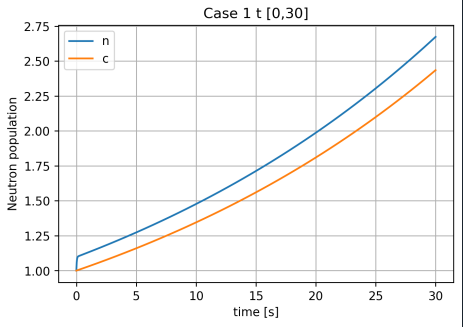
\includegraphics[scale=1]{Image_1_hw_4}
	\caption{Case 1 for n(t) of [0,30]}
\end{figure}

\begin{figure}[H]
	\centering
	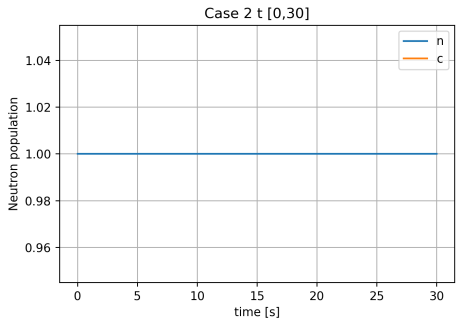
\includegraphics[scale=1]{Image_2_hw_4}
	\caption{Case 2 for n(t) of [0,30]}
\end{figure}

\begin{figure}[H]
	\centering
	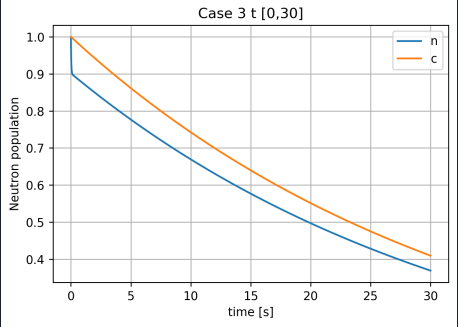
\includegraphics[scale=1]{Image_3_hw_4}
	\caption{Case 3 for n(t) of [0,30]}
\end{figure}

\begin{figure}[H]
	\centering
	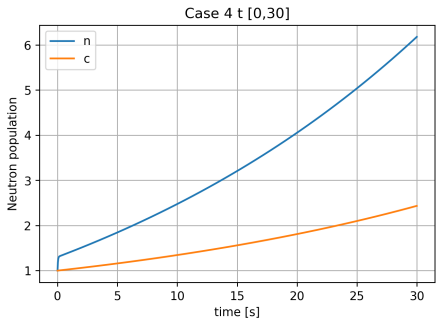
\includegraphics[scale=1]{Image_4_hw_4}
	\caption{Case 4 for n(t) of [0,30]}
\end{figure}

\begin{figure}[H]
	\centering
	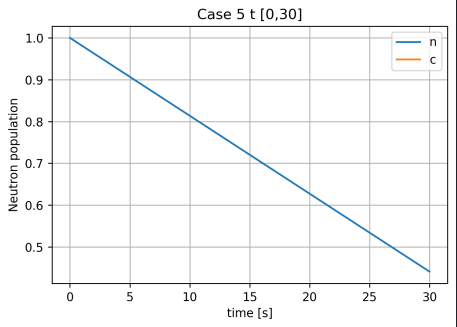
\includegraphics[scale=1]{Image_5_hw_4}
	\caption{Case 5 for n(t) of [0,30]}
\end{figure}

\begin{figure}[H]
	\centering
	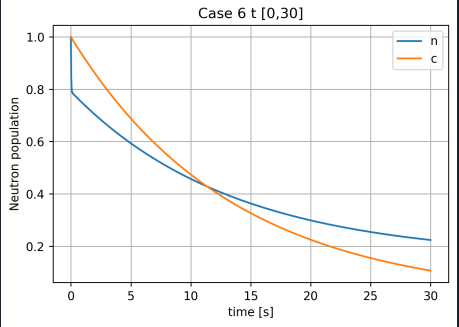
\includegraphics[scale=1]{Image_6_hw_4}
	\caption{Case 6 for n(t) of [0,30]}
\end{figure}

\begin{figure}[H]
	\centering
	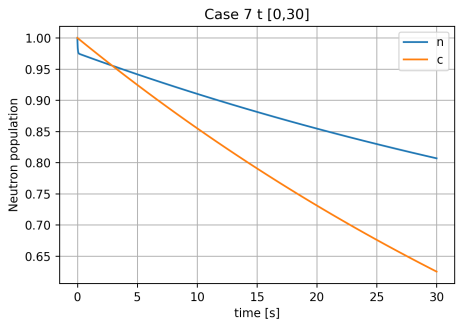
\includegraphics[scale=1]{Image_7_hw_4}
	\caption{Case 7 for n(t) of [0,30]}
\end{figure}

\begin{figure}[H]
	\centering
	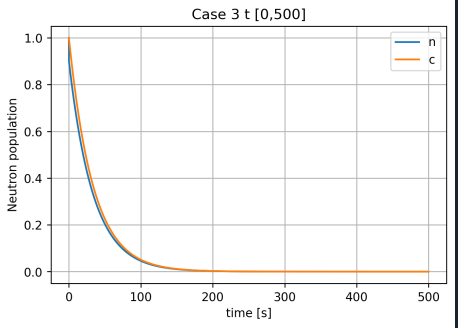
\includegraphics[scale=1]{Image_8_hw_4}
	\caption{Case 3 for n(t) of [0,500]}
\end{figure}

\begin{figure}[H]
	\centering
	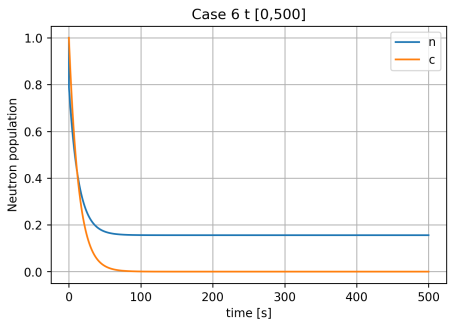
\includegraphics[scale=1]{Image_9_hw_4}
	\caption{Case 6 for n(t) of [0,500]}
\end{figure}

\begin{figure}[H]
	\centering
	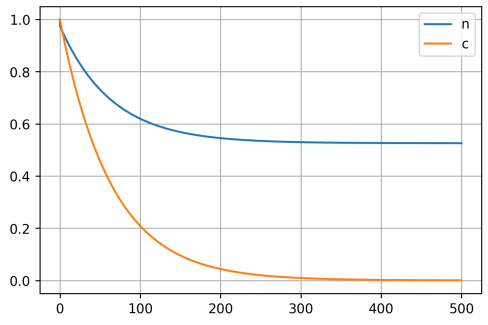
\includegraphics[scale=1]{Image_10_hw_4}
	\caption{Case 7 for n(t) of [0,500]}
\end{figure}

\begin{figure}[H]
	\centering
	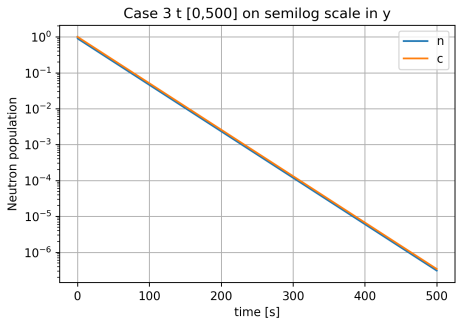
\includegraphics[scale=1]{Image_11_hw_4}
	\caption{Case 3 for n(t) of [0,500] with semilog scale Y axis}
\end{figure}

\begin{figure}[H]
	\centering
	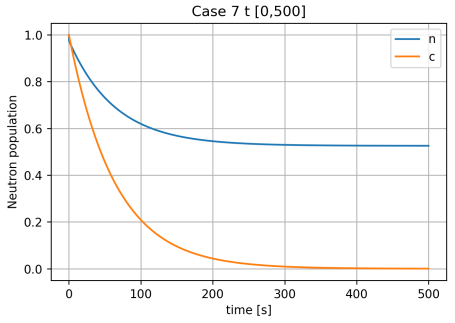
\includegraphics[scale=1]{Image_12_hw_4}
	\caption{Case 6 for n(t) of [0,500] with semilog scale Y axis}
\end{figure}

\begin{figure}[H]
	\centering
	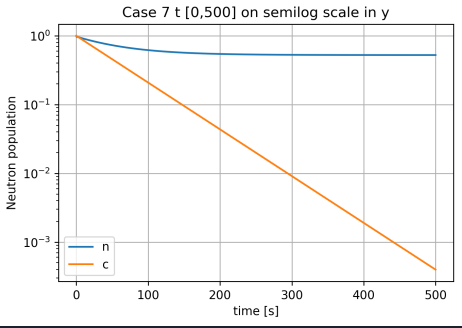
\includegraphics[scale=1]{Image_13_hw_4}
	\caption{Case 7 for n(t) of [0,500] with semilog scale Y axis}
\end{figure}


Plots for question 2. 
\begin{figure}[H]
	\centering
	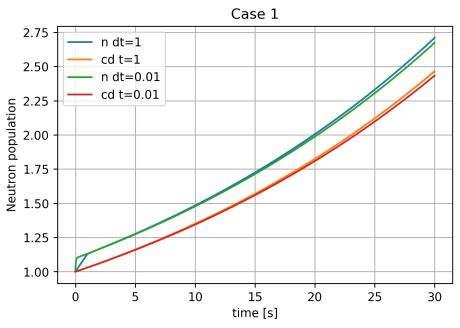
\includegraphics[scale=1]{Image_14_hw_4}
	\caption{Case 1 numerical solution}
\end{figure}

\begin{figure}[H]
	\centering
	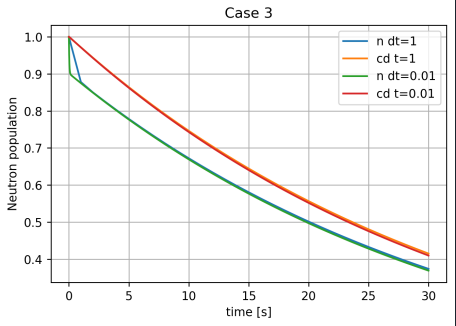
\includegraphics[scale=1]{Image_15_hw_4}
	\caption{Case 3 numerical solution}
\end{figure}

\begin{figure}[H]
	\centering
	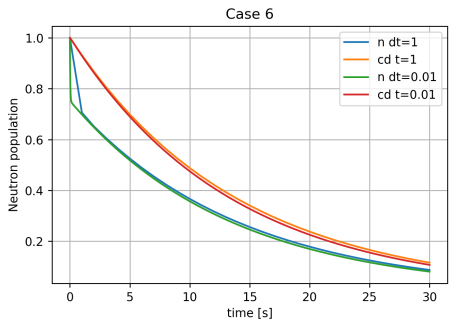
\includegraphics[scale=1]{Image_16_hw_4}
	\caption{Case 6 numerical solution}
\end{figure}

Question 3:
\begin{figure}[H]
	\centering
	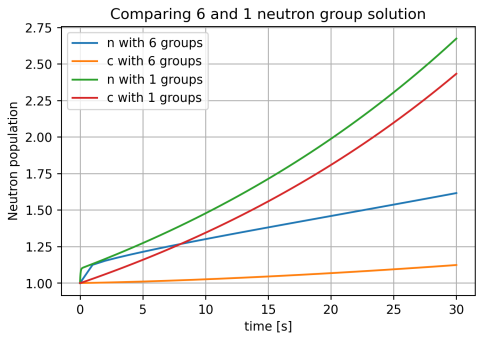
\includegraphics[scale=1]{Image_17_hw_4}
	\caption{Case 1 comparing numerical solutions with 1 and 6 neutron groups}
\end{figure}

\end{document}